\chapter{Programmation Scratch}  

Les ordinateurs sont des machines qui exécutent des programmes. On peut écrire des programmes dans différents \emph{langages de programmation}, par exemple \emph{Python}, \emph{C++}, \emph{Java}... ou encore \emph{Scratch}.\\

{\footnotesize
\begin{itemize}
\item Logiciel\footnote{Le logiciel \emph{Scratch} est librement téléchargeable : \url{https://scratch.mit.edu/scratch2download/}} : \emph{Scratch 2.0}
\item Matière concernée : mathématiques.
\item Compétences : 
        \begin{itemize}
        \item créer des nouveaux blocs avec ou sans paramètre d'entrée ;
        \item changer les arrière-plans de la scène ;
        \item changer les costumes du lutin ;
        \item créer puis détruire des clones d'un lutin. 
        \end{itemize}
\item Cette fiche est à réaliser :
        \begin{itemize}
        \item avant les vacances de Noël en mathématiques (séance 1) ;
        \item avant les vacances de printemps en mathématiques (séance 2) ;
        \item avant les vacances d'été en mathématiques (séance 3). 
        \end{itemize}
\end{itemize}
} % fin du footnotesize




\section*{Les années précédentes, vous avez appris...}

Les compétences listées ci-dessous ont été vues en classes de 6\up{e} et de 5\up{e}. Vous en aurez à nouveau besoin pour les activités de cette année. Si nécessaire, reportez-vous aux \emph{Fiches MITIC} des années précédentes pour revoir comment :  

\begin{itemize}
\item choisir et paramétrer l'objet lutin et l'objet scène (6\up{e}) ;
\item créer/insérer un nouvel objet (6\up{e}) ; 
%\item écrire un script comprenant mouvements, réponses à événement, boucles et sons (6\up{e}) ;
\item associer un script à un objet (6\up{e}) ;
\item utiliser la structure conditionnelle if (bloc \emph{si ..}) (6\up{e}) ; 
\item écrire un programme simple qui réponde à une problématique donnée (6\up{e}) ;
\item créer une variable et modifier sa valeur (5\up{e}) ;
\item utiliser la boucle for (bloc \emph{répéter $n$ fois}) (5\up{e}) ;
\item utiliser la structure if .. then .. else (bloc \emph{si .. alors .. sinon}) (5\up{e}) ; 
\item utiliser la boucle infinie (bloc \emph{répéter indéfiniment}) (5\up{e}) ;
\item lire un algorithme écrit sous la forme d'un \emph{flowchart} (5\up{e}) ;
\item écrire un programme à partir d'un \emph{flowchart} (5\up{e}).
\end{itemize}













%
%
%  S  É  A  N  C  E     I
%
%



\section{Séance 1 : Créer des nouveaux blocs}\label{ficheScratch4e1}

{\footnotesize \emph{(Auteur de cette séance : Thomas Morel, Institut Florimont)}}

\vspace{6pt}

\subsection{Pour bien démarrer...}

\subsubsection{Passer Scratch en langue française} 

Avant de commencer, il faut si nécessaire passer \emph{Scratch} en langue française :

\uneimageici{./images/scratch03/scratchFrancais}{.4\textwidth}

\subsubsection{Penser à enregitrer régulièrement}

Dès que vous avez ouvert un nouveau programme dans Scratch, sauvegardez-le au format Nom-date.sb3 : dans le menu \texttt{Fichier}, choisir \texttt{Enregistrer}. Pendant que vous travaillez, pensez à sauvegarder régulièrement votre travail (raccourci clavier \texttt{Cmd + s}).   

\uneimageici{./images/generales/clavierCmdS}{.4\textwidth}
\vfill

\subsection{L'activité demandée}

\vspace{10pt}

\boiteEnonceLarge{Le but de cette séance est de découvrir une notion importante en programmation : la notion de \emph{fonction}. Une fonction est une portion de code isolée que l'on peut appeler pour l'exécuter à chaque fois qu'on en a besoin. En \emph{Scratch}, une fonction est créée quand on crée un nouveau bloc. C'est ce que nous allons découvrir lors de cette séance. Nous allons suivre l'activité pas à pas afin de bien comprendre l'intérêt d'utiliser des fonctions.}


\subsection{Créer une ou plusieurs étoiles à 5 branches}

\subsubsection{Création d’une étoile à 5 branches}


À partir de l’algorithme ci-dessous, créer un script qui dessine une étoile à 5 branches.
\uneimageici{./images/scratch03/fonction/Scratch_Fonctions_01}{.6\textwidth}
Le résultat doit ressembler à ceci : 
\includegraphics[width=.9cm]{./images/scratch03/fonction/Scratch_Fonctions_02}.

\subsubsection{Création de plusieurs étoiles}

Modifier maintenant le script précédent afin d’obtenir la figure suivante (seules les étoiles sont à reproduire, les coordonnées sont mentionnées en rouge à titre indicatif).

\uneimageici{./images/scratch03/fonction/Scratch_Fonctions_03}{.6\textwidth}

Utiliser le bloc 
\includegraphics[width=2.5cm]{./images/scratch03/fonction/Scratch_Fonctions_04} pour positionner les étoiles aux bons endroits.
Que pensez-vous de votre dernier script ? Combien de blocs avez-vous utilisés ? Le script finalement obtenu est-il facile à comprendre ?

\subsection{Création d'un nouveau bloc}

Le script précédent comporte beaucoup de blocs et paraît donc, à première vue, compliqué à lire. On remarque également qu’une partie du code est reproduite quatre fois.

\uneimageici{./images/scratch03/fonction/Scratch_Fonctions_05}{.9\textwidth}


\vspace{1cm}

\begin{minipage}[c]{0.55\linewidth}
Afin de ne pas répéter le même code plusieurs fois, nous allons créer un nouveau bloc qui contiendra le code dessinant l’étoile, que nous nommerons : \emph{étoile} (figure ci-contre).

\vspace{6pt}

  \begin{itemize}
    \item \circled{1} Cliquer sur \texttt{Ajouter blocs};
    \item \circled{2} Cliquer sur le bouton \texttt{Créer un bloc};
    \item \circled{3} Entrer le nom de votre bloc (\texttt{étoile});
    \item \circled{4} Valider en cliquant sur le bouton \texttt{Ok}.
  \end{itemize}
\end{minipage} \hfill%
\begin{minipage}[c]{0.38\linewidth}
  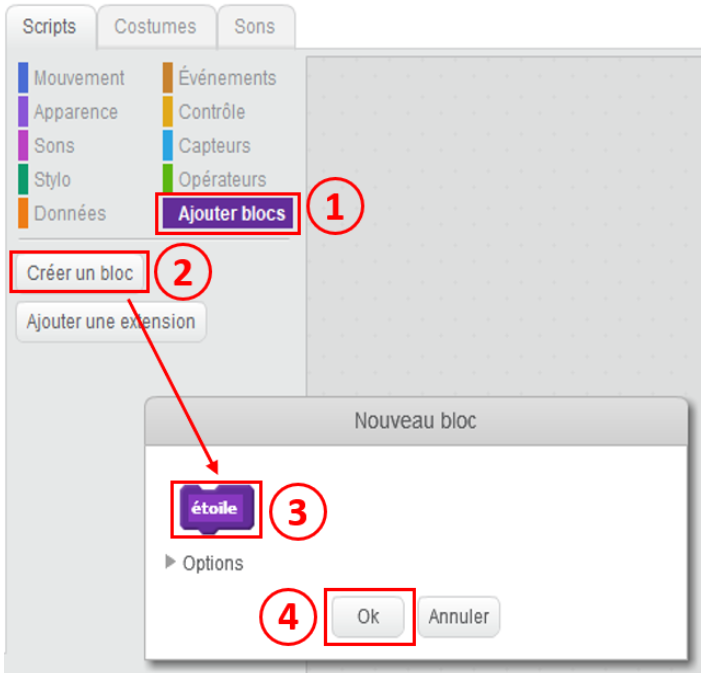
\includegraphics[width=0.9\textwidth]{./images/scratch03/fonction/Scratch_Fonctions_06}
\end{minipage}

Définir le bloc étoile de la manière suivante : 
 \begin{center}
 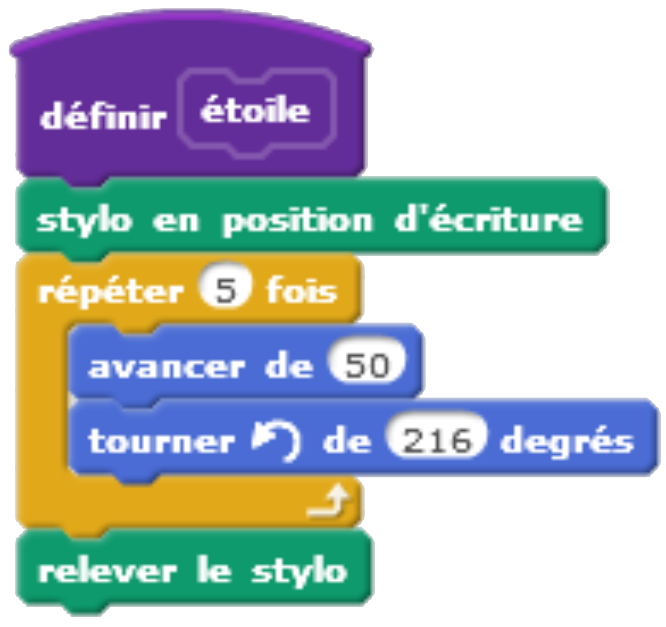
\includegraphics[width=0.25\textwidth]{./images/scratch03/fonction/Scratch_Fonctions_07}
 \end{center}

Il ne reste plus qu’à remplacer dans le script principal les parties de code correspondantes par le bloc  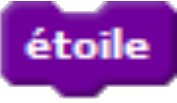
\includegraphics[width=1cm]{./images/scratch03/fonction/Scratch_Fonctions_08}. 

Vérifier que le nouveau script donne le même résultat que précédemment.

\cadre{Créer ses propres blocs évite de recopier du code qui apparaît plusieurs fois, ainsi le code devient plus court. Le programme ne sera pas plus rapide et le résultat sera le même, mais le code sera plus facile à écrire et à lire !}

\subsection{Paramétrer un nouveau bloc à l’aide d’une variable}

Il est possible de spécifier des paramètres en entrée d’un bloc créé par l’utilisateur afin de le rendre plus flexible. Plusieurs types de paramètres peuvent être utilisés en entrée du bloc :

\begin{itemize}
\item un nombre ;
  \begin{itemize}
   \item exemple : un paramètre «\,taille\,» pouvant prendre les valeurs 30, 40, 50... qui définirait la taille de l’étoile dessinée.
  \end{itemize}
\item une chaîne de caractères ;
  \begin{itemize}
     \item exemple : un paramètre «\,couleur\,» pouvant prendre les valeurs «\, rouge\,», «\,bleue\,»... qui définirait la couleur de l’étoile dessinée.
  \end{itemize}
\item une variable booléenne ;
  \begin{itemize}
    \item exemple : un paramètre «\,valeur\_défaut\,» pouvant prendre uniquement les valeurs 0 ou 1. Par exemple, quand valeur\_défaut vaut 1, les valeurs de taille et couleur pourraient être respectivement forcées à 30 et en bleu.
  \end{itemize}
\end{itemize}

Améliorons le bloc étoile afin qu’il puisse dessiner des étoiles de différentes tailles. Pour cela, il faut ajouter un paramètre d’entrée au bloc, que nous nommerons \texttt{taille}. Nous pourrons ainsi indiquer, au moment de l’appel du bloc, la taille de l’étoile.

\subsubsection{Ajouter un paramètre d’entrée de type nombre au bloc étoile :}

\begin{itemize}
\item Effectuer un clic droit sur le bloc étoile (\circled{1} sur la figure ci-dessous).
\item Dans le menu qui s’affiche, cliquer sur \texttt{éditer} \circled{2}.
\item Dans la fenêtre \texttt{Éditer} un bloc, dérouler le menu \texttt{Options} \circled{3}.
\item Choisir l’option \texttt{Ajouter une entrée nombre} \circled{4}.
\item Modifier le nom de votre paramètre d’entrée, choisir \texttt{taille} \circled{5}.
\item Cliquer sur \texttt{Ok} pour terminer \circled{6}.
\end{itemize}

\uneimageici{./images/scratch03/fonction/Scratch_Fonctions_09}{.6\textwidth}

\vspace{12pt}

Redessiner les 4 étoiles, chacune ayant une taille différente : 30, 40, 50, 60.

\vspace{12pt}

\subsection{Ajouter un commentaire à un nouveau bloc}

Pour faciliter la lecture du programme et comprendre rapidement à quoi sert le bloc créé, un commentaire peut être ajouté au moment de la définition du bloc.

\subsubsection{Ajouter un commentaire à la fonction étoile}

\begin{itemize}
\item Effectuer un clic droit sur votre bloc étoile (\circled{1} sur la figure ci-dessous).
\item Dans le menu qui s’affiche, cliquer sur \texttt{éditer} \circled{2} .
\item Dans la fenêtre \texttt{Éditer un bloc}, dérouler le menu \texttt{Options} \circled{3}.
\item Choisir l’option \texttt{Ajouter le texte du label} \circled{4} .
\item Entrer le commentaire :«\,dessine une étoile à la taille indiquée\,» \circled{5}.
\item Cliquer sur \texttt{Ok} pour terminer \circled{6}.
\end{itemize}

\uneimageici{./images/scratch03/fonction/Scratch_Fonctions_10}{.6\textwidth}



Vérifier que le commentaire apparait bien dans le script principal.

\cadre{Il est possible d’associer au bloc un ou plusieurs paramètres pour optimiser et adapter son comportement. Dans \emph{Scratch}, ces paramètres peuvent être de 3 types :
\begin{itemize}
\item type nombre ;
\item type chaîne de caractères ;
\item type booléen.
\end{itemize}

\vspace{6pt}

Les noms donnés aux paramètres sont très importants, puisqu’ils permettent au lecteur de tout de suite comprendre l’utilité du paramètre. Dans le cas d’un bloc compliqué, il est important d’ajouter un commentaire décrivant succinctement son utilité.}

\subsection{Pour aller plus loin...}

\subsubsection{Plus de paramètres}

Le script principal peut encore être réduit en intégrant les blocs 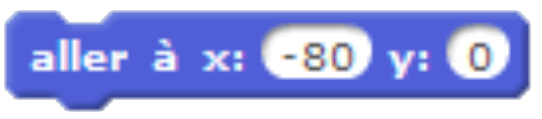
\includegraphics[width=3cm]{./images/scratch03/fonction/Scratch_Fonctions_11} dans un nouveau bloc créé.

\begin{enumerate}
\item Créer un nouveau bloc intitulé \texttt{étoile\&position} qui dessine une étoile en position (x,y) dont la définition est la suivante :
\begin{center}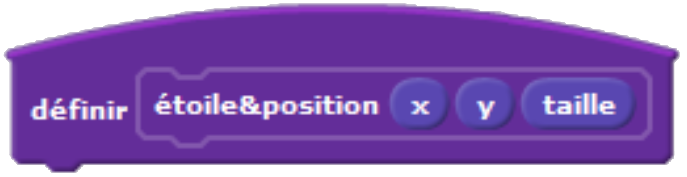
\includegraphics[width=5cm]{./images/scratch03/fonction/Scratch_Fonctions_12}\end{center}

\emph{Aide :} vous pouvez réutiliser le bloc \texttt{étoile} à l’intérieur du bloc \texttt{étoile\&position} si vous le désirez.

\item Modifier le script principal en utilisant le bloc \texttt{étoile\&position}.
\end{enumerate}

\subsubsection{Création d'un nouveau bloc «\,triangle\,»}

Définir la fonction \texttt{triangle} contenu dans le script ci-dessous qui permet d'obtenir la figure suivante :

\uneimageici{./images/scratch03/fonction/Scratch_Fonctions_13}{.8\textwidth}

\subsubsection{De plus en plus de côtés...}

Écrire le programme qui génère le résultat suivant :

\uneimageici{./images/scratch03/fonction/Scratch_Fonctions_14}{.5\textwidth}

\emph{Aide :} il est possible de créer une variable \texttt{n} qui contient le nombre de côtés de chaque forme pour ensuite l'utiliser dans la boucle.


\newpage 

%
%
%  S  É  A  N  C  E     II
%
%




\section{Séance 2 : Un clone de \emph{Flappy Bird}}\label{ficheScratch4e2}

\subsection{Pour bien démarrer...}

Dès que vous avez ouvert un nouveau programme dans Scratch, sauvegardez-le au format Nom-date.sb3 : dans le menu \texttt{Fichier}, choisir \texttt{Enregistrer}. Pendant que vous travaillez, pensez à sauvegarder régulièrement votre travail (raccourci clavier \texttt{Cmd + s}).   

\uneimageici{./images/generales/clavierCmdS}{.4\textwidth}

\subsection{L'activité demandée}

\vspace{10pt}

\boiteEnonceLarge{Le but de cette séance est de créer un jeu de type \emph{Flappy Bird}. C'est un jeu vidéo d'obstacles développé par Nguyen Hà Dong et sorti en mai 2013 (figure ci-dessous). Selon Wikipedia : \emph{«\,Le gameplay repose sur l'agilité du joueur, qui doit faire avancer un oiseau dans un environnement à défilement horizontal en tapotant sur l'écran tactile, tout en évitant des tuyaux présents en haut et en bas de l'écran. Les règles de jeu sont très simples : lorsque l'oiseau touche un tuyau ou heurte le sol, la partie est terminée.\,»}

\uneimageici{./images/scratch03/flappy/screenshotFlappy}{.6\textwidth}

Le jeu créé ici sera très simple : à vous de l'améliorer pour qu'il ressemble davantage à l'original ou à vos désirs !\\

Que devons-nous faire pour créer un tel jeu ? Première étape : se renseigner pour voir à quoi ressemble le jeu \emph{Flappy Bird}. Il est possible de trouver des vidéos sur \emph{Youtube}.
Voilà par exemple à quoi pourra ressembler notre clone de \emph{Flappy Bird} : sur la figure ci-dessous à gauche, le jeu en cours d'exécution et à droite lorsque le joueur a perdu.}


%\subsection{Création des éléments graphiques}

\boiteEnonceLarge{
\deuximagesici{./images/scratch03/flappy/screenshotFlappyClone01}{.8\textwidth}%
	      {./images/scratch03/flappy/screenshotFlappyClone02}{.8\textwidth}

On va utiliser une nouvelle fonctionnalité dans \emph{Scratch} : la création de différents \emph{costumes} pour un \emph{lutin} et la création de différents \emph{arrière-plans} pour une \emph{scène}.\\

Pour ce jeu il nous faut donc :
\begin{itemize}
\item des tuyaux (\emph{lutin} \texttt{Tuyau} possédant différents \emph{costumes}) ;
\item un oiseau (\emph{lutin} \texttt{Oiseau} possédant deux \emph{costumes}) ;
\item un décor (\emph{scène} possédant deux \emph{arrière-plans} différents). 
\end{itemize}
\vspace{8pt}
Voilà les différents éléments (voir plus bas des indications pour leur création) :

\begin{itemize}
\item une \emph{scène} qui contiendra comme premier \emph{arrière-plan} le fond d'écran (figure à gauche ci-dessous) et comme second \emph{arrière-plan} l'écran qui indique que le joueur a perdu (à droite ci-dessous) ;

\deuximagesici{./images/scratch03/flappy/scene03}{.6\textwidth}%
	      {./images/scratch03/flappy/scene04}{.6\textwidth}

\item un \emph{lutin} pour l'oiseau, qui contiendra comme premier \emph{costume} l'oiseau du jeu (figure à gauche ci-dessous) et comme second \emph{costume} l'oiseau après un crash contre un tuyau (à droite ci-dessous) ;

\deuximagesici{./images/scratch03/flappy/LutinOiseau03}{.3\textwidth}%
	      {./images/scratch03/flappy/LutinOiseau04}{.3\textwidth}

\item un \emph{lutin} pour les tuyaux, qui contiendra plusieurs \emph{costumes} pour chaque tuyau du jeu (figures ci-dessous).

\troisimagesici{./images/scratch03/flappy/lutinPipe00}{.1\textwidth}%
	       {./images/scratch03/flappy/lutinPipe00b}{.1\textwidth}%
	       {./images/scratch03/flappy/lutinPipe00c}{.1\textwidth}


\end{itemize}
}

\textbf{Pour obtenir de l'aide, rendez-vous à la page \pageref{aide_seanceScratch2}}



\subsection{Pour aller plus loin...}

Pour améliorer ce jeu, il est possible de :

\begin{itemize}
\item faire en sorte que si l'oiseau touche le sol la partie soit perdue ;
\item modifier la vitesse de chute de l'oiseau et sa vitesse de remontée ; 
\item ajouter des vies à l'aide d'une variable (le joueur commence avec trois vies puis en perd une à chaque fois qu'un tuyau ou que le sol est touché) ;
\item ajouter des sons (début du jeu, arrivée d'un tuyau, mort de l'oiseau, etc.) ;
\item augmenter le rythme d'apparition des tuyaux ; 
\item améliorer la qualité des graphiques ;
\item augmenter le nombre de costumes différents disponibles pour les tuyaux. 
\end{itemize}







%
%
%  S  É  A  N  C  E     III
%
%

\newpage

\section{Séance 3 : Tracer une fonction affine}\label{ficheScratch4e3}

\subsection{Pour bien démarrer...}

Dès que vous avez ouvert un nouveau programme dans Scratch, sauvegardez-le au format Nom-date.sb3 : dans le menu \texttt{Fichier}, choisir \texttt{Enregistrer}. Pendant que vous travaillez, pensez à sauvegarder régulièrement votre travail (raccourci clavier \texttt{Cmd + s}).   

\uneimageici{./images/generales/clavierCmdS}{.4\textwidth}

\subsection{L'activité demandée}

\vspace{10pt}

\boiteEnonceLarge{Le but de cette séance est d'utiliser \emph{Scratch} pour réaliser le tracé d'une fonction affine (fonctions mathématiques de la forme $y = a \times x + b$. Cette séance sera moins guidée que les deux précédentes : à vous de mettre en œuvre vos connaissances pour atteindre le but !

Les deux captures d'écran ci-dessous montre l'aspect du projet au moment où une donnée est entrée (figure de gauche) et après le tracer de la fonction (figure de droite).

\deuximagesici{./images/scratch03/traceFx/screenshot1}{\textwidth}%
	      {./images/scratch03/traceFx/screenshot2}{\textwidth}
}

 

%\subsection{Premiers réglages}

\boiteEnonceLarge{
Pour réaliser cette activité, la première étape consiste à sélectionner la scène et à choisir dans la bibliothèque des arrière-plans celui qui porte le nom \texttt{xy-grid} : il permet d'avoir à l'écran le repère dans lequel la fonction sera tracée.

\vspace{6pt}

Le programme utilise quatre variables qu'il faut créer : $a$ (contient la valeur du coefficient directeur de la droite), $b$ (contient l'ordonnée à l'origine), $x$ (valeur de l'abscisse) et $y$ (valeur de l'image de $x$).
}

\textbf{Pour obtenir de l'aide, rendez-vous à la page \pageref{aide_seanceScratch3}}

\subsection{Pour aller plus loin...}

Vous avez réussi ? Félicitations !

\vspace{6pt}

Pour améliorer votre programme, vous pouvez :

\begin{itemize}
\item cacher les variables $x$ et $y$ dont l'affichage à l'écran n'est pas utile ;
\item modifier la couleur et l'épaisseur du tracé ; 
\item modifier le programme pour qu'il trace une parabole (fonction de la forme $y=a \; x^2 + b \; x + c$) ;
\item modifier le programme pour qu'il trace une droite et une parabole. 
\end{itemize}


% AIDE
\newpage

\section{Aide pour réaliser les activités}

\subsection{Aide pour la séance 2}\label{aide_seanceScratch2}

\subsubsection{Construction des arrière-plans de la scène}

On va tout d'abord créer l'arrière-plan du jeu. Une fois \emph{Scratch} ouvert (figure ci-dessous), cliquer sur la scène \circled{1}, vérifier que l'onglet arrière-plans est sélectionné \circled{2}, choisir l'arrière-plan \no 1 \circled{3}, sélectionner le seau de peinture \circled{4}, puis l'option dégradé \circled{5}, choisir enfin une couleur \circled{6}. Terminer en cliquant dans la zone blanche pour peindre l'arrière-plan.

\uneimageici{./images/scratch03/flappy/scene01b}{.8\textwidth}
	      
On va ensuite créer l'arrière-plan qui doit être affiché lorsque la partie est perdue. C'est un nouvel arrière-plan appartenant à la même scène.

Pour ajouter un nouvel arrière-plan à la scène en cours, cliquer sur le pinceau \circled{1} (figure ci-dessous), choisir ensuite l'outil texte \circled{2} puis la police à utiliser \circled{3} et enfin la couleur \circled{4}. Terminer en cliquant dans la zone blanche pour écrire le texte souhaité. Il faut tirer sur les poignées qui apparaissent pour agrandir le texte jusqu'à la taille souhaitée, puis si nécessaire le déplacer à l'aide de la souris.

\uneimageici{./images/scratch03/flappy/scene02}{.6\textwidth}



À partir de maintenant il est possible de changer l'arrière-plan de la scène grâce au bloc suivant, disponible dans les blocs \texttt{Apparence} :

\uneimageici{./images/scratch03/flappy/basculeArrierePlan}{.4\textwidth}







\subsubsection{Construction des costumes du lutin \texttt{Oiseau}}

\emph{Remarque : pour gagner du temps, il est possible d'utiliser directement des lutins de la bibliothèque plutôt que de dessiner deux nouveaux costumes pour notre lutin. Dans ce cas, il faudra réduire la taille d'affichage du lutin afin qu'il soit plus petit à l'écran. Pour cela, utiliser le bloc \texttt{Mettre à ..\,\% de la taille initiale} disponible dans les blocs d'\texttt{Apparence}.}

\vspace{3pt}

\emph{Si des lutins de la bibliothèque sont utilisés pour définir les deux costumes du lutin \texttt{Oiseau}, alors rendez-vous directement au paragraphe \emph{Construction des costumes du lutin \texttt{Tuyau}}, \S\ \vref{costumesLutinTuyau}}.

\vspace{6pt}

Commencer par supprimer le lutin par défaut en effectuant un clic droit dessus puis en choisissant \texttt{Supprimer} (figure à gauche ci-dessous). Créer ensuite un nouveau lutin à dessiner en cliquant sur le pinceau (figure à droite ci-dessous).

\deuximagesici{./images/scratch03/flappy/lutinSupprime}{\textwidth}%
	      {./images/scratch03/flappy/lutinNouveau}{.7\textwidth}

La première étape est de créer un premier costume pour notre lutin. Pour cela, dessiner un oiseau (ou toute autre forme !) à l'aide des outils de dessin (ici l'outil ellipse et l'outil pinceau). \textbf{Attention !} L'oiseau doit être petit : observer que la zone de dessin a été agrandie à 400\,\% à l'aide de l'outil zoom (\circled{1} sur la figure ci-dessous).

\uneimageici{./images/scratch03/flappy/LutinOiseau01}{.6\textwidth}




La seconde étape consiste à créer un second costume pour notre lutin. Ce costume sera utilisé lorsque l'oiseau heurte un tube. Pour créer un nouveau costume, cliquer sur le pinceau (\circled{1} sur la figure ci-dessous), positionner le zoom sur 400\,\% puis dessiner le costume souhaité. 

\uneimageici{./images/scratch03/flappy/LutinOiseau02}{.6\textwidth}


À partir de maintenant il est possible de changer le costume du lutin grâce au bloc suivant, disponible dans les blocs \texttt{Apparence} :

\uneimageici{./images/scratch03/flappy/blocBasculerCostume}{.3\textwidth}


\emph{Remarque :} il est possible de modifier le nom des costumes ou des arrière-plans en utilisant la zone de saisie en haut de la zone de dessin. Il est également possible de changer le nom des lutins en sélectionnant le lutin puis en cliquant sur le \circled{$i$} (figure ci-dessous à gauche). Le nouveau nom peut alors est entrée dans la zone de saisie (figure à droite ci-dessous).

\deuximagesici{./images/scratch03/flappy/lutinChangerNom}{.3\textwidth}%
	      {./images/scratch03/flappy/lutinChangerNom2}{.9\textwidth}


\subsubsection{Construction des costumes du lutin \texttt{Tuyau}}\label{costumesLutinTuyau} 

\emph{Remarque : si vous avez changé la valeur du zoom de la zone de dessin lors de la création du costume du lutin à l'étape précédente, ne pas oublier de la ramener à 100\,\% avant de poursuivre ! Dans le cas contraire, vos tuyaux apparaîtront trop petits à l'écran pendant le jeu.}

\vspace{6pt}

Le but est de créer un nouveau lutin avec trois costumes différents correspondant à trois tuyaux différents comme montré sur la figure ci-dessous.

\uneimageici{./images/scratch03/flappy/lutinPipe01}{.6\textwidth}


Pour cela, créer un nouveau lutin à dessiner puis dessiner trois costumes différents. Pour dessiner un tuyau, le plus simple est de dessiner un grand rectangle rempli de couleur à l'aide de l'outil rectangle \circled{1} en choisissant le remplissage des formes créées \circled{2} (voir figure ci-dessous à gauche). À l'aide de l'outil gomme \circled{3} dont on règle la taille \circled{4}, couper en deux le tuyau (figure à droite ci-dessous).  

\deuximagesici{./images/scratch03/flappy/lutinPipe02}{.6\textwidth}%
	      {./images/scratch03/flappy/lutinPipe03}{.6\textwidth}

 





\subsubsection{Script associé à la scène}

Le script associé à la scène est très simple. C'est lui qui permet de compter les points gagné par le joueur. Le joueur gagne 1 point toutes les 2 secondes de jeu : pour gagner beaucoup de points, il faut donc rester en vie le plus longtemps possible !

\vspace{6pt}

Il faut tout d'abord commencer par créer une variable \texttt{SCORE}. Pour cela, cliquer sur les blocs \emph{Données} puis sur le bouton \emph{Créer une variable}. Lui donner le nom \texttt{SCORE}.

Le diagramme \emph{flowchart} suivant permet de construire le script associé à la scène :

\uneimageici{./images/scratch03/flappy/ScriptScene}{.5\textwidth}


On remarquera que la fin n'est jamais atteinte puisqu'une boucle \emph{Répéter indéfiniment} est présente (boucle infinie). Le comptage des points prendra fin lorsque le bloc \texttt{Stop tout} sera appelé (voir plus bas).





\subsubsection{Scripts associés au lutin \texttt{Oiseau}}

Deux scripts sont associés au lutin \texttt{Oiseau}. Le premier est très simple : il permet de faire «\,remonter\,» l'oiseau lorsque la touche \texttt{Espace} est pressée. Son diagramme \emph{flowchart} est donné ci-dessous.

\uneimageici{./images/scratch03/flappy/ScriptOiseau1}{.35\textwidth}

\vspace{3cm}

Le second script (voir page suivante) correspond au cœur du jeu : il permet de faire «\,tomber\,» l'oiseau en permanence et il laisse tourner le jeu jusqu'à ce que l'oiseau touche un tuyau. Une fois un tuyau touché, le script arrête le jeu, change le costume associé au lutin \texttt{Oiseau} afin de montrer qu'un obstacle est heurté et change l'arrière-plan associé à la scène pour afficher le message \emph{«\,Perdu !\,»}. Le diagramme \emph{flowchart} de ce script est donné ci-dessous. Attention, il faut créer une variable \texttt{JEU} qui prend la valeur \texttt{OUI} quand la partie est en cours et la valeur \texttt{NON} quand la partie est perdue.

\newpage 

\uneimageici{./images/scratch03/flappy/ScriptOiseau2}{.55\textwidth}


\subsubsection{Scripts associés au lutin \texttt{Tuyau}}

Le premier script à construire permet de créer un clone de tuyau, choisi au hasard parmi les trois costumes du lutin \texttt{Tuyau}. Comme il faut beaucoup de tuyaux en même temps à l'écran, on va créer des \emph{clones} du lutin qui existeront le temps de traverser l'écran de jeu. Les clones sont créés tant que la variable \texttt{JEU} a pour valeur \texttt{OUI}. Le diagramme \emph{flowchart} correspondant est donné ci-dessous :

\uneimageici{./images/scratch03/flappy/ScriptTuyau1}{.6\textwidth}


On remarquera que là encore la fin n'est jamais atteinte (utilisation d'une boucle infinie).

Le second script permet de contrôler un clone du lutin \texttt{Tuyau}. Ce script est appelé lorsqu'un clone est créé (bloc \texttt{Quand je commence comme un clone}). Il permet de positionner le clone à droite de l'écran, puis de le faire avancer petit à petit jusqu'à l'autre bord de l'écran. Arrivé à ce point, le clone est caché puis détruit. Voilà le diagramme \emph{flowchart} correspondant :

\uneimageici{./images/scratch03/flappy/ScriptTuyau2b}{.75\textwidth}


Il est possible de modifier la vitesse avec laquelle les tuyaux traversent l'écran. Au choix, vous pouvez :
\begin{itemize}
\item modifier la valeur $-5$ par une autre ;
\item utiliser une valeur aléatoire en lieu et place de la valeur $-5$ ;
\item créer une variable vitesse qui change de valeur en fonction de la variable score, ce qui permet de faire avancer les tuyaux de plus en plus vite et rend le jeu plus difficile au fur et à mesure que le temps passe.
\end{itemize}


% SEANCE 3

\subsection{Aide pour la séance 3}\label{aide_seanceScratch3}

%\vspace{6pt}

Tous les scripts qui seront écrits concernent le lutin : il faut donc sélectionner celui-ci avant de commencer à programmer.

\vspace{6pt}

La script principal (script qui va appeler tous les autres) sera celui de la figure ci-dessous. Il contient des nouveaux blocs que vous allez créer (inutile donc de les chercher tant que vous ne les avez pas créé !).

\uneimageici{./images/scratch03/traceFx/fonctionPrincipale}{.25\textwidth}

\emph{Remarque :} le bloc \texttt{cacher} permet de faire disparaître le lutin.

\vspace{6pt}

La figure ci-dessous présente les trois nouveaux blocs à créer.

\uneimageici{./images/scratch03/traceFx/nouveauxBlocs}{.8\textwidth}



\subsection{Création du bloc \texttt{entrée des données}}

\uneimageici{./images/scratch03/traceFx/blocEntreeDonnee}{.27\textwidth} 

Ce nouveau bloc doit permettre de demander à l'utilisateur d'entrer une valeur pour la variable $a$ et une valeur pour la variable $b$. À chaque fois la réponse de l'utilisateur est stockée dans la variable correspondante.

\vspace{6pt}

\emph{Aide :} Lorsqu'on utilise le bloc \texttt{demander ... et attendre}, la réponse de l'utilisateur est stockée dans la variable réponse (figure ci-dessous).

\uneimageici{./images/scratch03/traceFx/questionReponse}{.5\textwidth}




\subsection{Création du bloc \texttt{calcule f(x)}}

\uneimageici{./images/scratch03/traceFx/blocCalcule}{.2\textwidth} 

Ce nouveau bloc est très simple : il range la valeur $a \times x + b$ dans la variable $y$.




\subsection{Création du bloc \texttt{trace f(x)}}

\uneimageici{./images/scratch03/traceFx/blocTrace}{.2\textwidth} 

Ce nouveau bloc permet de tracer tous les points de la fonction, c'est-à-dire tous les points de coordonnée $(x\,;y)$ où $y=a\times x + b$. Il faut commencer le tracé avec la valeur $x=-240$ (bord gauche de l'écran), puis augmenter la valeur de $x$ de 10 en 10 (inutile de tracer tous les points).







